%%%namn p filien Raport felix andrad
%%% datum 2011 02 15
%%%%% mallen: nedladdad frn http://www.ee.iitb.ac.in/~trivedi/LatexHelp/latexsample.htm


%% This LaTeX-file was created by <guest> Sun Jan  3 14:45:46 1999
%% LyX 0.12 (C) 1995-1998 by Matthias Ettrich and the LyX Team

%% Do not edit this file unless you know what you are doing.


%%%%%%%%%%%%%%%%%%%%%%%%%%%%%%vikitga ting start
\documentclass[12pt]{report}
%%%%%%%%%%%%%%\documentclass[12pt]{article}
\usepackage[T1]{fontenc}
\usepackage{geometry}
\geometry{verbose,a4paper,tmargin=15mm,bmargin=30mm,lmargin=30mm,rmargin=20mm}
\usepackage{graphics}
\usepackage{setspace}


%%%%%%%%%%%%%%%%%felix inlagg
\usepackage[applemac]{inputenc}
\usepackage[swedish,english]{babel}
\usepackage{amsmath}
%\usepackage[retainorgcmds]{IEEtrantools}
\usepackage[gs]{graphicx}
%%%%%%%%%%%%%%%%%felix inlagg

\setcounter{secnumdepth}{5}
\setcounter{tocdepth}{5}
\onehalfspacing

\makeatletter


%%%%%%%%%%%%%%%%% LyX specific LaTeX commands.
\newcommand{\LyX}{L\kern-.1667em\lower.25em\hbox{Y}\kern-.125emX\spacefactor1000}
\makeatother
\renewcommand\bibname{References}
%%%%%%%%%%%%%%%%%%%%%%%%%%%%%%





\begin{document}
%\bibliographystyle{plain}


%%%%%%%%%%%%%%%%%%%%%%%%%%%%%%frsta sidan
\begin{titlepage}
\thispagestyle{empty}
\vspace*{0.7cm}
{\centering	 
\large
{\Large\bf Tjuv och polis}\\
\vspace{3cm}
\bf{Ph.D. kandidatarbete}\\
\vspace{0.25cm}
\vspace{0.1cm}
\vspace{1cm}
\it
by \\
\vspace{.5cm}
\rm
\selectlanguage{swedish}
{\large \bf {Felix Blumenberg}}\\
{\large \bf {person nr1}}\\
{\large \bf {Fredrik Bberg}}\\
{\large \bf {880312}}\\
{\large \bf {Mats Malmberg}}\\
{\large \bf {person nr3}}\\
\selectlanguage{english}
\vspace{1cm}

{\it{under the guidance of}} \\
\vspace{.5cm}

\hspace{.05cm} {\large \bf {Doctoral Student Johan Thunberg}}\\
\hspace{.05cm} and\\
\hspace{.05cm} {\large \bf {Professor, Ph. D Xiaoming Hu}}\\
\vspace {0.5cm}
\vspace {0.5cm}
%\iitbseal\ \\

\begin{figure}[h]
%\hspace{6cm}
%\vspace{5cm}
%{\centering {\includegraphics{iitlogo1.ps}}\par} LOGO!
\end{figure}

Department of mathematic optimization \\
Royal Institute of Technology KTH, Sweden\\
{\centering
\hspace{6.5cm}Feb 2011}
}
\pagebreak
\end{titlepage}
%%%%%%%%%%%%%%%%%%%%%%%%%%%%%%






%%%%%%%%%%%%%%% %%%%%%%%%%%%%%% tv abstrakt olika sprk olika sidor
\selectlanguage{english}
\vspace{2in}
\begin{abstract}
In this paper heursitic algorithms are developed for the pursuit evasion problem in polygonal enviroments. In this problem, continuous trajectories shall be constructed for a group of pursuers, searching for an evader, in such a way that the evader is guaranteed to be seen at some time during the search.
%The problem consists of constructing continous trajectories for a group of pursuers, searching for an evader, in such a way that the evader is guaranteed to be seen at some time during the search.
Three fundamentaly different heuristic methods are considered: tabu search, genetic algorithms and greedy methods. The result is three heuristic algorithms. Two algorithms are readily implemented in ANSI C, yielding solutions of high quality compared to previous work. The report attains and evaluates statistics on runtime of the algorithms. The algorithms are compared considering the quality and efficiency for a vast amount of randomly generated enviroments.\\
\\ \textbf{Key-words}: Pursuit and Evasion, Heuristic algorithms, tabu search, greedy methods, genetic algorithms.
\end{abstract} 

\selectlanguage{swedish}
\vspace{2in}
\begin{abstract} 
\selectlanguage{swedish}
I detta arbete utvecklas heuristiska algoritmer f�r problemet ``pursuit and evasion in polygonal enviroments''. Problemet best�r i att konstruera kontinuerliga banor f�r en grupp av s�kare, s�kande efter en inkr�ktare, s� att inkr�ktaren garanterat blir sedd vid n�gon tidpunkt i s�kningen. Tre i grunden olika heuristiska metoder behandlas f�r att f�rs�ka skapa algoritmer kan finna l�sningar p� problemet. Resultatet �r tv� k�rbara algoritmer som snabbt ger l�sningar av h�g kvalitet. De tre heuristiska metoderna vi har valt att behandla �r tabus�kning, genetisk algoritmer och giriga algoritmer. Arbetet tar fram och utv�rderar statistik p� k�rtider och l�sningens kvalitet f�r ett stort antal slumpm�ssigt genererade omr�den. \\
\\Nyckelord: Heuristik, algoritmer, tabu, girig, genetik, multiagent pursuit and evasion, implementation, kth, kandidatarbete, NP-sv�rt, kungliga tekniska h�gskolan.

\end{abstract} 

\selectlanguage{english}
%%%%%%%%%%%%%%%%%%%%%%%%%%%%%%


%%%%%%%%%%%%%%%%%%%%%%%%%%%%%%% innehllsfrteckning
\pagenumbering{roman}
\tableofcontents{}

%%%%%%%%%%%%%%%%%%%%%%%%%%%%%%%
\listoffigures
\newpage
\newenvironment{mydef}[1]{\begin{definition} #1 \mbox{\\}
\rm}{\end{definition}}
%%%%%%%%%%%%%%%%%%%%%%%%%%%%%%%


%%%%%%%%%%%%%%%%%%%%%%%%%%%%%% arbetet
\pagenumbering{arabic}

%%%% 	vill du lgga  in ngot dokument ngon stans lgg det i rtt ordning nedan
%%%%     samt anvnd nedstende document som mall nr du skirver

\chapter{Introduction}

\section{Objective}

The aim of this paper is to construct heuristic algorithms that solve the  pursuit \& evasion problem for a two dimensional polygonal environment. The origninal pursuit \& evasion problem is fully formulated in chapter two. Informally it can be formulated as``given an static environment with obstacles, and a specific number of pursuers, ensure that an evader cannot exist within the environment''. An algorithm providing an optimal solution already exists \cite{paper2}. In practice this algorithm is not very applicable though, since even for small areas the time complexity is considerable. This is where heuristic methods could provide interesting results. By sacrificing the optimality, our aim is to use heuristic methods to try and find a sufficiently good solution within a reasonable computational time. Appart from the previous work of Johan Thunberg \cite{paper2}, we have not found any related work where heuristics is applied to the problem. 
\section{Background}

\subsection{What is optimization?}
Optimization is a mathematical discipline for solving various types of problems. The aim is to find the best available value of some objective function, given a defined domain.% Refer to other literature?
The mathematical theory behind optimization offers a variety of methods to solve a wide range of problems. To approach these problems and, find a solution, it is important to identify the characteristics of the problem considered. Relevant distinctions can be made by studying the problem's complexity. Complexity is strongly related to the computational time. There are many different complexity classes of problems, but two of the most fundamental are the P and NP.

\subsection{P \& NP problems.}
%skriva om hela sektionen??
The distinction between these two reveals the difficulty of our problem. This will only be a brief description, for a more detailed and interesting description please see \cite{NP}.

P is the set of problems which can be solved by a deterministic Turing machine using a polynomial amount of computation time.
Cobham Edmonds thesis holds that P is the class of computational problems which are "efficiently solvable" or "tractable". In practice, some problems not known to be in P have practical solutions, and some that are in P do not, but this is a useful rule of thumb.

NP refers to Non-deterministic Polynomial time, and can be intuitively described as the set of problems for which, a found solution can be verified to actually be the correct solution, using a deterministic Turing machine using a polynomial amount of computation time.

A set of descriptions that leads one to wonder whether
\begin{equation}
P = NP
\end{equation}

In what the essence is:
Suppose that solutions to a problem can be verified quickly. Then, can the solutions themselves also be computed quickly?
Or stated differently, does it exist such an algorithm that can calculate such a solution quickly?
An unsolved question considered by many to be the most important problem in the field of computer science. 

Within the class NP there are a few subclasses one of them are called NP-hard 
Related work has stated that the problem studied in this report are in fact of the class NP-hard \cite{paper1}, % Is it paper one?
and hence the chances of finding an algorithm that produces an optimal solution in polynomial time are greatly reduced. As stated above it is still an open question whether such algorithms actually exist for NP problems. 

\subsection{A near optimal solution.}
As mentioned in \cite{paper1} the problem under consideration is at least NP-hard. The consequences of this is that the chances of finding an optimal solution within reasonable computional time are seen to be very low. Thus we are imposed to sacrifice optimality, in order to gain computational effictivity. This sacrifice opens a large spectrum of possible approaches to the problem.


\subsection{Heuristic methods}
Heuristic methods are a branch of methods used in computer science and mathematics to make relevant guesses to find solutions to a problem. In general heuristic methods does not provide optimal solutions. Though sometimes, for specific situations, it can be proven that a certain heuristic algorithm's solutions are optimal. Also, there is no general way of proving whether a heuristic algorithm provides an optimal solution. Despite this fact heuristic methods often provide extremely efficient and relevant algorithms. Very often they reduce the computational time needed for a solution greatly. There are even several occasions where a heuristic method is prefered to an analytic method. A few examples are:
\begin{itemize}
\item When there is no known algorithm for solving a specific problem, a heuristic is the only way to approach a solution.
\item A algorithm can sometimes be difficult to implement. Heuristics can sometimes be used instead because they are easy to implement and known to produce good results.
\item When the problem is too difficult to solve efficiently and quickly with analytical methods. A heuristic method could overcome that and give an acceptable but probably not optimal solution.
\end{itemize}

The last point corresponds to the problem we are dealing with.
\chapter{Environment}
The chapter gives a description of the simulation environment we have created. Presenting how we created it, why we needed to create it and motivation of the choices made.\\

First we give an short overview of the parts that are in the enviroment, and a definition of in/out data. Motivating all our choices made concerning limitations in the enviroment, and also describing positive features of our enviroment.

\section{Generator}
The environment generator has length, width and number of obstacles as input. By construction each subarea is convex. The generator also tests for the total area to be connected, which guarantees a feasible environment.\\\\
Every environment created can be considered to be built of squares. This results in that diagonal edges will not be created, but since a diagonal can be created by a line of obstacles if the resolution is high enough, that should not be a loss of generality. \\\\
\\
\section{Node network}
Our node-network generator takes a matrix as input and generates a graph network, which is to be used by our algorithms.\\
The array can either be generated, se previous section, or hand-made.\\
\chapter{Methods}
In this report it was decided to use the heuristic concepts from greedy methods, tabu search and genetic algorithms to construct the algorithms. These methods has been intentionally chosen so that each method strongly differs in its characteristics from the other two. Greedy methods are local and deterministic in their approach. Both tabu search and genetic algorithms are stochastic and global in their approach, but they differ significantly in how they examine and construct feasible solutions. The reason for this decision was to examine if some conclusion could be made about if any specific characteristics would be favourable for solving our problem. 

\pagebreak
\section{The genetic algorithm approach}
Genetic algorithms are based on the idea of evolution, that the most suited individuals tend to live longer and reproduce. 
\subsection{Description of genetic algorithm}
In Genetic Algorithms, or GA's, a population is simulated in an artificial world using a combination of reproduction, gene crossover and mutation, with a given goal for the population to achieve. As in nature, a population consisting of individuals are used. As a simplification, each individual has one chromosome, containing one or more genes. During each generation, individuals are selected and paired for reproduction, and their genes are combined to form new children.\\
\\
Due to the need to simulate the population and evaluate individuals, often multiple times, GA's are not well suited for all kind of problems. When there exists an analytical solution it may be better to use that. However, if the problem can be simulated, both problems without analytical solutions and problem with complicated analytical solutions can be handled by GA's, although it is never guaranteed to give an optimal solution.\\
%% Variations / Generational / Steady-state
There are different ways to implement genetic algorithms, with variations in how each step is performed. This yields many different versions of genetic algorithms. Firstly there are two different kinds of GA's, steady-state and generational, where steady-state maintains and alters one population and generational replaces an old population with a new one.
Figure~\ref{GeneticFlowChart1} shows a flowchart of a genetic algorithm.
\begin{figure}[!h]
	\centering
	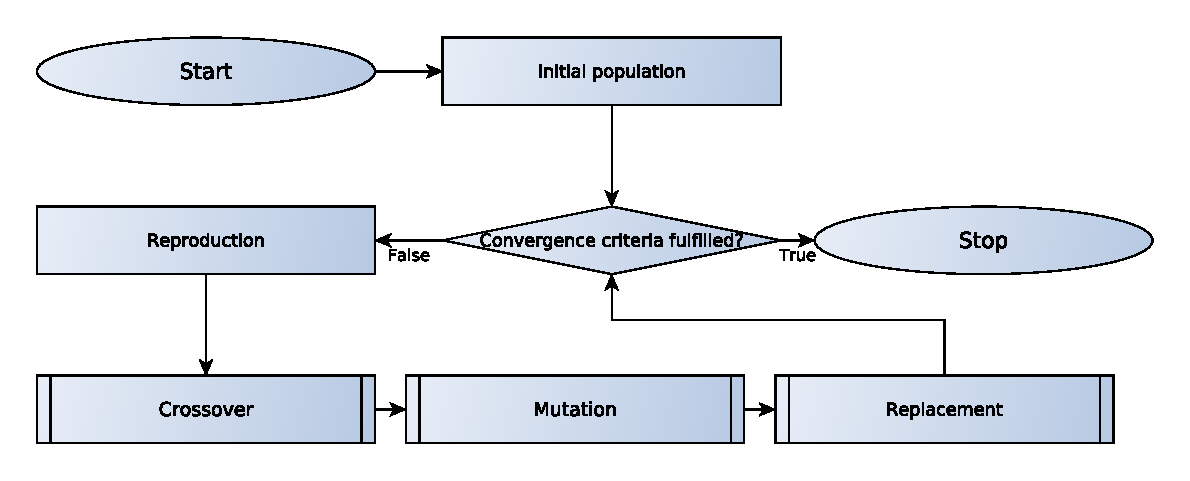
\includegraphics[width=\textwidth]{chapter_4_methods/GeneticFlowChart-Generic}
  	\caption[Flowchart of a genetic algorithm]
  	{Flowchart of a genetic algorithm}
	\label{GeneticFlowChart1}
\end{figure}
%% Initial population
\\At first an initial population has to be obtained, either an existing set of solutions or created in some way.\\
%% Evaluation / Fitness function
To be able to evaluate and compare different individuals, a fitness function is used. The fitness function should calculate a score for an individual, depending on how fit the individual is in relation to the goal.\\
%% Breeding
Evolution is performed using a breeding step during which two individuals are selected and used to create two new individuals. The creation is done first by crossover and then by mutation.\\
%% Selection (parents)
For selection, there are different methods but five of them are Fitness Proportionate Selection, Random Selection, Fit-Fit, Elite selection and tournament selection.\\
In Fitness Proportionate Selection, of which Roulette Selection is one example, the probability of choosing a more fit individual is higher than to select a less fit individual.\\
In Random Selection, the probability to be selected is equal for all individuals. \\
With Fit-fit, at each step the two most fit individuals are selected. In the next step the next two most fit are selected.\\
In Elite selection the best individual is chosen. This selection procedure should be used in combination with another selection method.\\
Tournament selection chooses a number of individuals stochastically, and then take the best of them.\\
\\
%% Crossover
For Crossover there are different methods, a few of those are n-point shuffle crossover, uniform crossover and variable crossover.\\
\\
%% Mutation
\\Mutation is important in GA's since it makes sure that all the search space can be reached, even if the initial population did not cover all of it. It can be implemented as 'bit-flip', if the gene is binary encoded, where a 0 is changed to 1 and 1 to 0.\\
\\
%% Replacement
When breeding has been completed, in order to not increase the population size, a replacement has to be performed. For this there are several methods, such as Weak Parent, Both Parents, Weakest Individual and Random.\\
In Weak Parent, a weaker parent is replaced by a stronger child.\\
In Both Parents, the children replaces the parents.\\
In Weakest Individual, the children replaces the two weakest individuals in the population, if the children are fitter.\\
In Random, the children replaces random individuals in the population.\\
\\
%% Termination
To make sure the algorithm ends at some point, a termination condition has to be used, for instance a maximum number of generations, a limit in fitness sum, a median fitness, best individual or worst individual.\\
With Fitness sum, the algorithm will terminate when the sum of the fitness for the population is less than or equal to a specified value.\\
With Median fitness, a range for the fitness is specified.\\
With best individual, the algorithm will terminate when the minimum fitness drops below a convergence value and thereby guarantee at least one good solution while saving time.\\
With Worst Individual, the algorithm will terminate when all individuals in the population has a fitness value lower than the convergence value.\\
\\
%% Encoding
To adapt genes to computers, an encoding has to be used.  According to literature \cite{GAHandbook1} binary encoding is the fastest encoding, where each gene is encoded as 0 and 1, but there are also integer encoding and string encoding.\\
%%%% Development process of the genetic algorithm
\subsection{Development process of the genetic algorithm}
The first idea to use  was to use an existing framework for Genetic Algorithms, such as LibGA or GAUL, to save time on programming. Due to the implementation of the libraries, for this application it was determined to be faster to write a new implementation.\\
\\After reading parts of the source code of existing libraries and Johan Thunberg's Boolean Control software \cite{paper1} for ideas, a first attempt to a program was written. The first version was a boolean control network, where feasible solutions were generated by using a random function to generate numbers between 0 and 4 to indicate if the pursuer were to move left, right, up, down or stand still. For each pursuer, an integer based encoding was used, which was easy to implement and debug compared to binary encoding. Each digit in the gene is called an allele, following the notation from \cite{GA-ai}. It was thereafter extended to a generational GA instead of steady-state, because of easier implementation and a more clear termination condition in number of generations. \\
%% Fitness
At first a simple fitness function with two variables was used \eqref{fitness1}, S4 which is the number of nodes in state 4 and \textbf{step} which is the total number of steps taken to minimize S4.
\begin{equation}\label{fitness1} (1+S4+steps) \end{equation}
A change of selection procedure, see next paragraph, made it necessary to switch to a function which was to be maximized \eqref{fitness2},  where the numerator was used to scale the fitness value closer to positive integer values.
\begin{equation}\label{fitness2} \frac{1000}{(1+S4+steps)} \end{equation}
The final version of the fitness function was a simplified version of \eqref{fitness2}. By using the total number of nodes, called Nodes,  and the maximum allowed steps, called MaxSteps, the fitness function was limited to positive integer values, which should be easier for a computer to calculate.
\begin{equation} \label{fitness3}Nodes-S4+MaxSteps-steps \end{equation}
%% Selection
\\For selection, Random, Tournament  and Fitness Proportionate Selection were considered, all three in combination with elite selection to avoid loosing the best solution found. Random selection is the easiest to implement and was first used to create a working GA, but it was replaced with Tournament selection as it gives a more fit individual an advantage. In the final version a Fitness Proportionate Selection was used, which gives more fit solutions an even greater advantage and thereby helps the population converge even faster. Elite selection was used to keep track of the two best solution each generation.\\
%% Crossover
\\To make the crossover operation easy to implement, a version of n-point crossover was used. One path from each pursuer was used alternating from each parent.\\
%% Mutation
\\Due to the integer encoding, and node network representation, 'bit-flip' was not easily implemented. Instead a gene is selected by a random function, and thereafter a random allele is chosen to be replaced. When an allele is replaced all following alleles are generated again to make sure the path generated is feasible.
%% Replacement
\\To make sure the overall fitness of the population increased, a weak parent replacement was used.\\
%% Parameters
\\At first a population size of 400 was used, which was what worked best after 10 trial runs at 5x5, in combination with a limit of 100 generations and 200 steps/alleles. Mutation frequency was set to 5\% after testing different values, which is more than the often used value in literature \cite{GAHandbook2} of 1-2\%, but still not very large. The parameters varied, and due to the increasing computation time with increasing population size a relatively small population of a maximum of 2000 individuals was used, in combination with a high mutation rate of 75\% and a maximum of 800 generations. This was in order to cover a large search space when working with environments larger than 5x5 nodes, without having an population size of over 4.000 which at some attempts took over 10 minutes for a single generation. The final version of the program had a more dynamic population size and step length, see next subsection.

\subsection{The genetic algorithm of our problem}
The final version of the genetic algorithm had a maximum population of 2000 individuals and 600 steps\footnote{depending on the size of the environment the maximum number of steps was set between 50 and 600 }, but during initialization the population size and step length was limited to a lower value if possible. This was done by creating an initial population of 400 individuals, evaluating each and see if any solution clears the environment. If it does, the maximum step length is limited to the number of steps used, and the population is incremented by 100 individuals to increase the probability of having a diversity in the population.
\begin{figure}[!h]
	\centering
	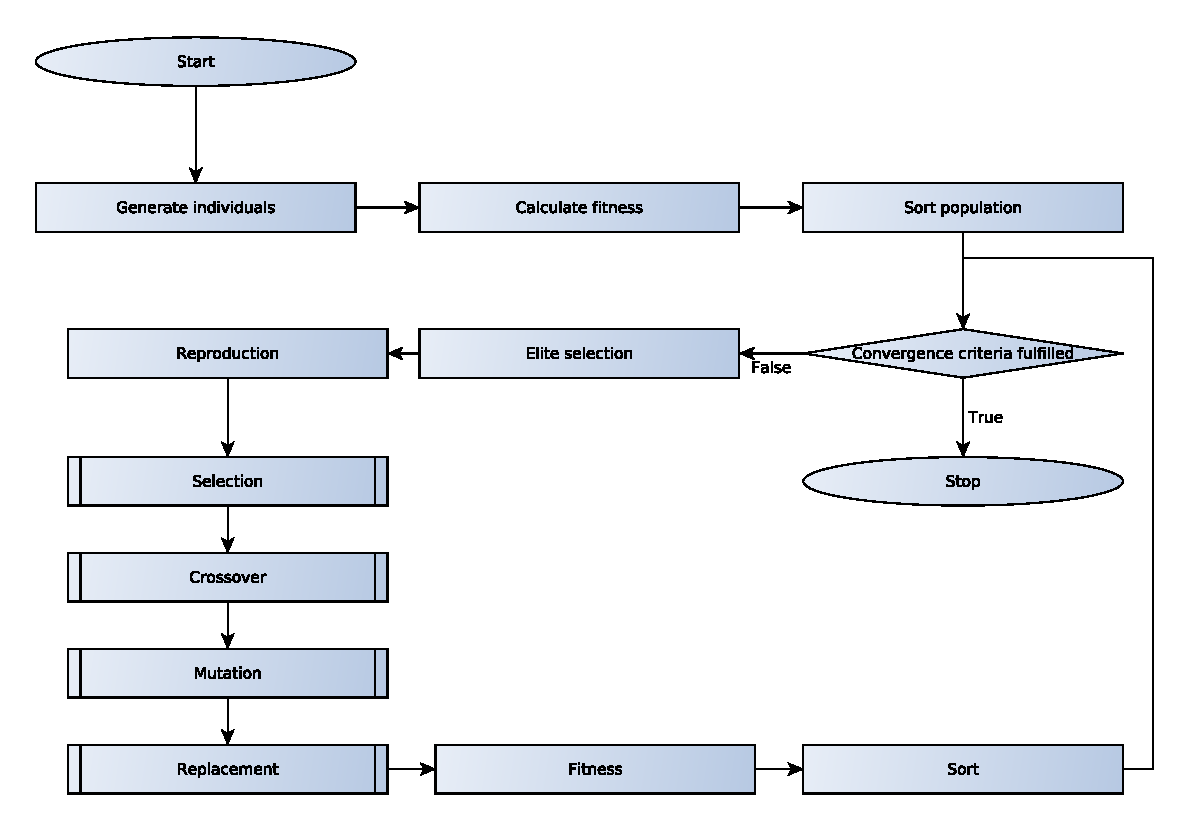
\includegraphics[width=\textwidth]{chapter_4_methods/GeneticFlowChart-Algorithm}
	\caption[Flowchart of the implemented genetic algorithm]
	{Flowchart of the implemented genetic algorithm}
\end{figure}
%% Initial population
\\As written in the previous subsection the initial population was generated by a random function, which gave each pursuer a sequence of alleles that represented each step.
%% Fitness 
Each individual was evaluated using \eqref{fitness3}, and sorted by fitness in decreasing order, which facilitated selection.
%% Breeding
The two individuals with the best fitness value was added to the new population, and thereafter the selection process selected individuals for breeding. Fitness proportionate selection was used, in which the sum of the fitness value was calculated and a random number between 0 and the sum was generated. The fitness was thereafter added for each individual until that number was reached, and that individual was selected. This was repeated to select a second parent. The crossover was copying genes alternating between each parent, so that two different children were created. A mutation step was performed with 75\% probability, where an allele from one of the gene was replaced as described in the previous subsection. Finally the best individuals of the parents and children was  placed in the new population, and the step is repeated until a new population of the same size as the previous was created.
%% Termination
As a termination criteria the fitness score of up to 99\%\footnote{Values between 50\% and 99\% was used} of the population was compared. If the individuals had completely cleared the environment and had an equal fitness score, the algorithm was terminated. As 99\% is a very high convergence criteria, it was only used for small environments to avoid premature termination. As a second termination criteria the maximum number of generations was set to 800, to make sure the algorithm would terminate even if no solution was found.
\subsection{Our implementation of the genetic algorithm}
The algorithm was implemented using C. Every time a random value was to be obtained \begin{verbatim} ((int)((double)rand() / ((double)RAND_MAX + 1)*SCALE_FACTOR)); \end{verbatim} was used, which generates a number in the range [0,SCALE\_FACTOR). As a random seed number \begin{verbatim} srand(time(0))\end{verbatim} was used. No alternative random functions were evaluated.\\
For sorting the population, quicksort was used \cite{quicksort}.\\

\section{The greedy algorithm approach}
\subsection{Description of greedy algorithms.}
Greedy algorithms can be either itterative or recursive. In most cases a itterative algorithm can be reformulated as a recursive one and vice versa. For simplicity we will consider the greedy algorithms itterative unless stated otherwice. In each itteration the algorithm has a set of possible alternatives on how to to push the algorithm towards a solution. A so called "cost function" designates a cost to each alternative. At the end of the itteration the alternative with the best cost, be it maximum or minimun, is choosen as a part of the solution. \\
\\It is not guaranteed in general that greedy algorithms provide optimal solutions. Also there is no general way of determining wether an greedy algorithm provides an optimal solution or not, but there are two very important properties that usually helps to determine if an optimal solution can be provided. These are the greedy-choice property and the optimal substructure property (referens [10] kap 16.2). The greedy choice property states that an global optimal solution can be arrived at by making locally optimal choices. In other words, at each itteration a choice can be made without reconsidering previous itterations. The optimal substructure property states that an optimal solution can be expressed as a sum of solutions to subproblems. If these two properties are fullfilled, then a solution can be constructed by summing optimal subsolutions. Hopefully this is an optimal solution, but if one want's to be shure more rigorous proofs are needed. 

%By formulationg algorithm recursion one it is easier to apply induction for a formal proof of a solution to be optimal. 
%If the greedy algorithm is recursively formulated we can describe the two properties as follows: Suppose that we have a optimization problem P, and that there exists an optimal solution S. Also, suppose that P has optimal substructure and greedy choice properties. Then a solution S* is given by the optimal subsolution $p_0$ plus the solution to the remainding problem P'. Following this line of thought again for P' one gets that $S*=p_0 +p_1 + solution (P'') =>S*=sum(p_i)$ 

%the problematics, as always with recursion, is to find a proper generic question. so that it is solvable, and so that it actually returns the answer we excpect to find.
  
%when constructing the algorithm for a problem P one starts out by finding some part of the solution. formulate this as a generic step and loop. This is exactly how the algorithm for the multi pursuer problem has been constructed.

\subsection{Development process for the greedy algorithm.}
When constructing a greedy algorithm one often starts by finding some part of the final solution and then extend this to find a correct generic question for recursion. As in the examples given in the online lectures \cite{online lecture} the question and answer yielding a correct algorithm may not be intuitive. In the approach of creating the greedy algorithm for our problem we assume that it is possible to find the best movement strategy by locally finding the best next step until we arrive at a totally secured state of the enviroment. So the generic question would informally be "what is the best next step for the pursuer team?". In the development process for the greedy algorithm there has been a couple of candidates to answer this question. At last only one seemed like a good choice, presented in section 3.
\\
\\The first candidate "alorithm 1" was to make the secured area our objective function. In each itteration we consider the next move for each hunter in the team, and try to move the whole group so that we maximize the secured area (the objective function). We would then have a objective function and constraints due to the enviroment and pursuer positions. This ought to be possible to solve as some sort of linear programming problem. After consideration this naive approach presented several drawbacks. First off, for many enviroments it is sometimes nessecary to let go of secured areas. This could not be alowed by algorithm 1 with a greedy approach. Also there are a lot of cases where the best move is not an increase in secured area, but rather guarding or transportation to strategic positions. This was allowed, but not very likely to be chosen by the algorithm due to the greedy approach. It was thus realized that the algorithm somehow must look further than just the head on approach of targeting the secured area.
\\
\\The next candidate was an attempt to extend the formulation of algorithm 1 to have dynamic constraints, hereon called algorithm 2. The idea was to introduce some sort of tactics to the pursuer team, and thus make the group cooperate in a favorable manor. For each pursuer a certain tactic would be given, corresponding to constraints to the objective function. In order to formulate these constraints, we needed more information. Here the idea of introducing different areas was first met. The common vision of the pursuer team divides the enviroment into several subareas, not visible by the team. Depending on the state and geometry of these subareas each hunter was supposed to either guard, secure or divide a given subarea. This is dynamic information about the enviroment, thus giving dynamic constraints for each pursuer. In this case it was problematic to find a general formulation of how to choose a tactic, and how to formulate these tactics as constraints for the objective function. Also there were to many special cases and intuition involved for a possible implementation.
\\
\\For the third candidate the idea was to use the extra enviromental information about the non visible areas and somehow apply this to a simple greedy cost function. By designating costs to each feasible tile it would be easy to make a greedy choice. By construction each hunter can in general move to at most four tiles or stand still. Thus by giving each of these five alternatives a value that quantifies how good the move is we'll find the best over all strategy of the team. With this setup the objective function for each itteration is to maximize the sum of the tile-values that each pursuer moves into. So, how does one quantify what  a good tile is? The obvious answers such as field of vision and state are, by them self, insufficent information for a good algorithm. But by using the dynamic information of the areas, resulting from the pursuers vision, we can find more parameters to quantify the best move. In order for the pursuer team to spread out and cooperate we designate a unique area for each pursuer to approach. This is done by adding a value to the tiles that give the shortest path for a specific pursuer to approach its designated boundry. Furthermore we add a value to all moveable tiles depending on their unique guarding properties of priorized areas. The algorithm will now make good tactical descisions, given that the added values are correctly adjusted. 
\\
\\This last candidate is was used as a basis for the final algorithm.To arrive at the algorithm presented in section 3 several examples has been tested manualy on random enviroments. In the manual execution the aim was to delete all human intuition from the algorithm and strictly quantify the valuation of the tiles with simple numbers or questions, suitable for a computer. A more in depth explanation of the algorithm is given in the next section.
%fram hit har jag kollat....
\subsection{The greedy algorithm for our problem}
In this section the final greedy algorithm will be explained in detail, step by step. Before the algorithm is started a prefunction is executed to find all static information on the enviroment. Since these static conditions only need to be evaluated once, and can be evaluated at any time they are not an interesting part of the algorithm itself but will be described in the section 4.1.4 concerning the implementation.
\begin{figure}[!h]
	\centering
	\includegraphics[width=\textwidth]{chapter_4_methods/greedy_uml3.jpg}
  	\caption[Flow chart of greedy algorithm]
  	{Flow chart of greedy algorithm}
\end{figure}

The algorithm is written in an itterative way, and a overview is given by the flow chart in figure 4.1. In each itteration the algorithm finds and executes the best move for each pursuer. Each step will now be described in detail.
%\begin{wrapfigure}{r}{0.4\textwidth}
%\centering
%\includegraphics[width=0.4\textwidth]{chapter_4_methods/Example_enviroment1.jpg}
%\caption{Text wrap around figure}
%\noindent
%\hrulefill
%\label{test}
%\end{wrapfigure} 

\begin{enumerate}
\item{} The input for each itteration is the path taken so far. For the first itteration this corresponds only to the starting positions of the pursuers.
\item{} At the beginning of each itteration a decision is made whether to make another itteration or not. An itteration should be executed if the enviroment is not all secured and if the breaking conditions are not met. The breaking conditions are given by the main program running the algorithm, so that if no solution can be found the algorithm will abort in due time.   
\item{} Here we find the total field of vision of the pursuers team. This will divide the enviroment in seen and unseen areas as in figure 4.2.(figur som visar geometri f�r omr�den. needed??)   
\item{} All areas not visible by the pursuer team are given a priority, a boundry and if possible an extended boundry. The priority is determined by the geometric properties of the area. If the area is secured it is only relevant to guard its boundries, thus secured areas are not to be designated in any of the preceeding steps. Contamined areas can be categorised in four different types. In descending order of priority they are:
\begin{itemize} 
\item{}Areas with only one boundry, where the whole area can be seen from the boundry tile.
\item{}Areas with several boundries, where the whole area can be seen from some boundry tile. 
\item{}Areas with only one boundry tile, but who can not be fully seen from the boundry.
\item{}Other areas.
\end{itemize}
A boundry to an area is by construction seen by some pursuer. If the area can be seen from a boundry we can usually extend this boundry so that all tiles from which the whole area can be seen are part of the ``extended boundry''.  
\item{} In this step a table of possible choices for the pursuers is created. As mentioned above the secured areas should not be a part of the table. The extended boundries are to be used when measuring the shortest distance to a boundry for a pursuer. This is because our aim is to \emph{see} the area, and the extended boundries usually provides shorter distances for the pursuers.
\item{} Given the table created we now want to choose as many elements as there are columns, since the columns corresponds to pursuers. The choice is to be made in such a way that there is at most one element chosen from each row and column and so that the sum of the chosen elements is minimized. Also there is a constraint that the rows corresponding to areas that can be fully seen from their boundries must be chosen if possible. A chosen element $c_{i,j}$ corresponds to designating the area of row i to the pursuer of column j. If there are more pursuers than areas, an area can be designate to more than one pursuer but all areas must be designated to at least one pursuer. 
\item{} Given the designation made in the previous step, for each pursuer there is at least one path of shortest distance to the designated boundry. For each pursuer,  add a value $\alpha$ to the tiles being the first step of the paths with the shortest possible distance to the designated boundry.
\item{} For each pursuer:
\begin{itemize}
\item{} Add a value $\beta$ the tile being closest to any contamined area. 
\item{} Add a value $\gamma$ to the tiles where the boundries that are uniquely seen by this pursuer can still be seen. Here the secured areas are to be considered as well.
\item{} Add a value $\delta$ to the tiles where the boundries to areas that are secured, or that can be seen from its boundries, are still seen by the pursuer.
\item{} Add a value $\epsilon$ to the tiles where the pursuers has the largest field of vision.
\end{itemize}
\item{} In the previous steps we have now added at most five values to each tile in the proximity of each pursuer. For each pursuer find the tile with the largest sum and move the pursuer into this tile.
\item{} When the movement is made, update the states of the enviroment correspodingly. save the path taken so far. Return the updated states and the path taken so far to the start of the algorithm. 
\end{enumerate}
\subsection{Implementation of the greedy algorithm.}
Due to a combination of time pressure and shortcommings in the programming language C, the implementation of the greedy algorithm failed. Even though a ready-to-run implementation was not made, many parts of the implementation were finished.\\
\\In the prefunction all the needed static information about the enviroment is evaluated and saved to a struct. 
\begin{verbatim}
struct Greedy{
int SolutionPath[]; 
struct Node NodeMatrix[][];
int BreakCondition[];
HashTable; 
}
\end{verbatim}
The solution path is an array where index 0 contains the number of pursuers, index 1 contains the itterations made (set to zero by the prefunction), and the rest of the indices are the coordinates for each pursuer. The NodeMatrix is the graph created by the simulation enviroment described in chapter three. The break condition is simply an integer to describe the maximum allowed itterations. Since the algorithm needs to know the distance and the path between two tiles and this is saved into a hashtable. To find the shortest path and the distance between two tiles the A-star algorithm is used. 

FIND THE COMPLEXITY OF A-STAR!!! Dijkstra:  algorithm of $O(\vert v \vert^2)$ , a-star is special case of dijkstar? 
%pregreedy:
%a-star to find the distance and the path between any two tiles. describe complexity
%hashtable to access shortest distance in a fast manor, key: (from to)
%descride the greedy struct contents and motivate.


The implementation of the algorithm described in the previous section calls for the usage of a couple of interesting algorithms to solve some of the steps. In step four we want to find the interior of all areas. This was implemented by first taking any tile not part of the pursuers vision. Make a breadth first search to find and mark all the interior points of this area. Find a new unmarked and unseen tile and execute another breadth first search. Repeat this until all tiles not visible by the pursuer team are marked. The breadth first algorithm's time complexity is $O(\vert V \vert + \vert E \vert)$ \cite{adk8}, where V is the number of vertices in the graph and E is the number of edges.\\
\\For step six in the algorithm (the assignment) the implementation is designed to exaust all possible combinations and then pick the combination giving the smallest sum. The combinations are found by usage of a queue (first in, first out). Here one could try to use the Hungarian method \cite{hungarian} instead, but since the size of the table is usually not very large this algorithm seemed like overkill.  





\section{The Tabu search method approach}

\subsection{Description of Tabu search method}

Tabu search is a metaheuristic\footnote{ metaheuristic: simmular to heuristic  with the add on that it solves the problem iterativly}  optimization method, designed to search for the global optimum. Meaning that the method, figuratively, has the ability to climb out of a local minimum, and then explore other parts of domain.
There are several solutions on how this abilitie can be acquired. Tabu search uses a so-called tabu list, intended to bring former visited areas in to the domain to be forbidden, "tabu", to return to.
Tabu search has a few konseptiual blidnigblocks and basic ideas, easy to understand but with widely varying difficulty to implement. Konsept which, if well implemented will give you a highly sofisticeated search algorithm.
The core bildingblock is as mention before the tabu list. The ability to render a surten regen or moves tabu lets ous creeate a search startegis bilt on the infromation at hand, in a given moment, and prier experienses of the search. Hens tabu search is all about coming upp with intelegent roules, that vill sett a spesific move to be tabu or not. 
Another key bildingblock is the tabu overriding mechanism, in the litetur named as the aspriation criteria [glover]. Its jobb is to check wheter a certain move should be approved even if it initaly var sett to be tabu. In addisen this mens that the existens of the apriation criteria alowes the the tabu list to be more strikt. (And the search a lott faster.)

With these two key blidnigblocks one can construct almost any type of logic strucktur. 
Which makes the tabu search an highly implementebal and adaptive method.
A logic structure  that can be built with these two is the one wich is the actual main idea behind the tabu search method.
To anderstand this grundtanke of tabu search one rely needs to get to therms with the random aspekt of heuristik search. 
The tabu list and aspiration criteria only deels with the random selekted path/moves/solutions, this offcors meens that the current solution maight not be a good one. But and this is the nutchell: 

LEMMMA1 START 1
a solution/move produst out of a strategy tells something abut the problem at hand, indebendet wheter the achul solution/move wör a good or a bad one.
LEMMMA END 1

A insait that at furst glans might seem somwhat basic but if implemented in a good way yeelds powerfull ressoults.

In this deskripten certain aspect of the tabu search method has nowingly bin neglekted to make it more anderstandebul. 
 
To gain claraty a generalaised tabu serch algorithem will dawnbelow be deskribed in a step by step sevdo cod fachen (flochart)

Word convention: 
Compleet solution = a sett of moves that have soulved the problem
Incompleet solution = a sett of moves that vill not soulve the problem
feasible solution = a sett of moves that have not yett soulved the problem or have not yett bin evalueted whter it is a compleet/incomplete solution.


1
Obtiain feasible soultion or solutions. this are often generated randomly  =>2
2
Evaluation of the feasible solution
If it is a compleet solution, save it. Update tabu list and aspiration criteria accordingly. =>5
If it is a new best compleet solution, save it. Update  the tabu list, the aspiration criteria and the stopping criteria accordingly. =>5
If it is a incomplete solution, maby save it. Update tabu list and aspiration criteria accordingly. =>5
If still a feasible solution => 3
3
check it against the tabu list:
If not tabu. Update tabu list and aspiration criteria accordingly =>5
If tabu => 4
4
check it against the aspiration criteria:
Override the tabu list. Update tabu list and aspiration criteria accordingly => 5
not override the tabu list=>5
5
Check stopping criteria:
If reached => 6
If not =>1
6
Terminat algorithem, return final solution



\subsection{Development process of the Tabu search algorithm}

The develepment prosses of the tabu serch algoritem vill her be fromulated and the tjojses taken along the rood expland.
This prosses hade a few key fechers being: it had a strikt dead line and inexperiens among the programers, hens the dead line agen. This forced the prosses in a direktion that the idees needed to be somewhat esaly implemented. 

Letts star by analysing the random genereting of moves a.k.a. feasible solution, see step 1 in figur [flochart].
The furst cross roued was encontered when the dessiton of generat one feasible solution at a time, was tacken, insteed of a sett of feasible solution. The reasen behyend this cooyes was that the genetic algorithem allrady hade gone down the path of generating a sett of feasible solution \footnote{ refering to poppulation se sechten???}. And diversity was desired.
The second cross roued, on the subjekt of generating moves, was wehter to generet one move or a seris of moves to generat a new feasible solution. This dessition was harder to make, sinns aider chois seemed to generat highly prommising but wery diffrent algorithems. The implimentation of making a seris of moves would be an intermeedieat between the two choueses of the furst crossroed. And resoult in receding horizon [referens johan papper] aprooch where one hade to ader: 
\begin{enumerate}[(a)]   
\item produse a larg sett of seris of moves to later sort bay fittnes, then chouse one to check against the tabu list and aspiration critera.
\item generat a singel seris of moves to check against the tabu list and aspiration critera.
\end{enumerate}
Both alternetives would probebly have jeelded prommesing algorithems, but the fakt that the tabu list and aspriation critera then would have needed more of a analysing tipe ability i.e. more difficult to implement resulted in that this path was skrapt. This ment that the one move one feasible solution approach came out ahead.

This setheled we can now move forverd to view the ideas of the tabu list:
In the begingn of the development the ideas fluricht. Sex different rouls wher evalueted   

\begin{enumerate}

\item fore one feasible solution save the past X number of moves for each prosuer and render theese moves tabu to be return to.


\item Not alow moves that results in X number of lost secured areas

\item Geometri baesed tabus for kritikal areas:
\subitem mening areas of corridor like karakter would not be needed to be walkt down if one saw its end point. Or if one hade an area whit a obstical that one could walk around, hens it needs two persoer to secure,  it would be tabu to go about to try secure it alone. And finaly if one hade a tree like corridor system, going about to solve it would only be alowed with the right amount of prosuers.

\item Work togheter:
\subitem somewhat simmular to tabu roul (3) but with the addon that two persouers never rely need to see each other only chare vissebal arias. A more of a genneral roule that would need to be weighted in the aspriation criteria

\item high Walued areas:
\subitem trying to inkoperat the idea of  LEMMA1 in the way that the path taken, areas walkt appon in a compleet solution chould be given a walu bonus. Or if you look appon it from the ather angel, areas not walkt appon could be sett to be tabu 

\item low Walued areas:
\subitem an incomplete solution my have a seris of moves that have bin konsentrated on a spesific regen for to long, hens one could give this areas a walu penalty.

\end{enumerate}

All this tabus was needed to be rankt, given a priorety level that would be weight in the aspiration criteria. Also many of the tabu rules listed abow needed sume sort of worst case senario handeling, to awoyed the algorithem of getting stuk.

This said lets diskuss the aspiration critera:
As anderstud from the text abow the aspiration critera needs to inkoperat a lott. As a start it needs to have the abilety of cheking if an area is of high or low walu. Which then means that the evaluation step in figure [flochart1] needs a fitness calculation function that would depend on the area visited and the shape of the feasible solution.
Sad to say this aspiration criteria, would need an overwhelming amount of work hours to implement. Thus this advanced aspiration criteria was scrapped for a simpler one. This also means that tabu rules (3), (4) and (6) no longer could be implemented. Tabu rule (5) got simplified to: areas not walked upon where set to be tabu. More about tabu rule (5) later.
The more simple aspiration criteria, in the end, only came to be more of a worst case scenario handling, to avoid the algorithm of getting stuck.

Tabu rule (5):
When this rule first was implemented the idea was that X number of past complete solutions were analyzed, to check which areas had been walked upon, at least ones, and render the rest tabu.
The problem was however that this wasn’t strict enough. So X was set to one. Which intern led to the arising of another problem?
The problem that arouse was that the algorithm now, under certain circumstances, was too hasty in returning a final solution.
The problem was partially solved by some new stopping criteria and “go about it again criteria”.

That was the development process of the tabu search algorithm, the final version can be viewed in figure [ ] and also discussed in the next section.

 








\subsection{The Tabu search algorithm for our problem}

Pseudo code dvs förklaring av tabuvilkoren.
Ffllllllllllooooooooooooooooooooooooooooo


1
Obtain feasible solution by going one step with each pursuer randomly =>2
2
Evaluation of the feasible solution
If it is a new best complete solution, save it. Update the tabu list, the aspiration criteria and the stopping criteria accordingly. =>5
If it is an incomplete solution. Update stopping criteria accordingly. =>5
If still a feasible solution => 3
3
Check it against the tabu list:
If not tabu. Update tabu list and aspiration criteria accordingly =>5
If tabu => 4
4
Check it against the aspiration criteria:
Override the tabu list. Update tabu list and aspiration criteria accordingly => 5
Not override the tabu list=>5
5
Check stopping criteria
If reached = >6 
If not =>1
6
Terminate algorithm, return final solution


\subsection{Implementation of the Tabu search algorithm}


Skiva ner pretabu
Tabu 
Uppdelning etc

Beskrivning av sättningen av parametrarna List K list 
Alla konstiga utskrifter grejen


Hur dom jävla tabuvilkoren hanterades ,ordningen av koden.




\chapter{Results}
Statistics, tables and a description of the tables. Also motivation to why we have chosen these tables etc.\\\\
Results for MILP\footnote{Mixed Integer Linear Programming, see \cite{paper3}} evaluation could also be added here.
\chapter{Discussion}

This chapter contains analysis of the data collected when running the algorithms and conclusions made during the process.

\section{The simulation}
The simulation environment developed was usable, but is not without limitations.\\
As the simulation environment can not merge tiles into one node, something that could be usable for certain geometries such as hallways, the memory usage is proportional to the number of tiles.\\
The graph approach meant that no more nodes than necessary was examined in each step.\\
To read environments from files makes the simulation environment usable for many kinds of environments. New environments could either be generated or added by hand.\\
%utv�rdera f�rdelar och nackdelar som simuleringsmilj�n besitter.
	%f�rklara visions tillkortakommande
	%kan inte mergea, kr�ver mycker minne
	%graph-approach var bra ide?
	%applicerbar pga filskrivning
\section{Analysis of the simulations}
First off it should be noted that when varying the size of the enviroment certain parameters of the algorithms had to be adjusted. For enviroments of intermediate size a correct adjustment of parameters yielded solutions of significantly higher quality. For larger enviroments it was necessary in order to attain any solution at all. We found no analytical way of adjusting the parameters. A good understanding of the implementation in combination with intuition and testing usually solved the issue. This does not exclude the possibility that there might be a more descisive approach. In fact, based mainly on our intuition, it is most probable.\\
\\As seen in the table \ref{SimData}, given in the previous chapter, for small enviroments both algorithms efficiently provides solutions of high quality, even with a small amount of pursuers. The optimality of the solutions on the randomly generated enviroments is not proven, but it's likely that the provided solutions in most cases are optimal. This assumtion is motivated by the fact that the quality of the solutions rarely differs and the path length is typicaly only a few steps long. It should be noted that the average computational time for these solutions is 3 milliseconds for the tabu search algorithm and 37 milliseconds for the genetic algorithm. These are highly efficient results compared to related work \cite{paper1}.\\%n�mn och j�mf�r manhattan resultat
\\When the size of the enviroment is increased the solutions found are less probable to be optimal. This assumption is motivated by the fact that the quality of the solutions now vary strongly. Also the computational time severely increases with the size of the enviroment. An interesting observation though is to compare how the average computational time for the two algorithms changes as the difficulty increases. The tabu search algorithm is highly efficient if it is able to find a first complete solution. But when running on the bigger areas the average time diverges. On the other hand the genetic algorithm provides reasonable average computational times, and is more reliable to find some solution even for difficult enviroments.\\
\\By combining an indepth understanding of the implementation with the data aquired the following conclusions, and fundamental differences, can be made on the implementation of the algorithms. The tabu algortithm is strongly dependent on finding a complete solution of sufficient quality, in order to be efficient. The reason behind this is that a maximum step length is set dynamicaly by the complete solution found, and tiles not visited in this solution are rendered tabu. Thus, with a complete solution of bad quality there are still a vast amount of aternative paths to consider, which in turn affects the efficency.\\
\\The genetic algorithm does not have the same dependency of finding a complete solution, due to its reproduction properties. This motivates the more robust results on efficency for larger areas, compared to the tabu algorithm. 		
\section{Starting positions}
%l�sningskvalitet starkt beroende av startpositioner.
	%formulera tydligt vilka startf�rh�llanden som avses i problemst�llning hos framtida arbeten.
	%vi har slumpstart, varf�r? vad kan vi se?
	%bed�m kvalitet p� given l�sning utifr�n omst�ndigheter.
	
\section{When do the algorithms fail?}	
%n�r skiter det sig och varf�r?

\section{Future work}
%future work:
	%f�rb�ttra v�rat arbete programmeringsm�ssigt
	%implementera ideer uteblivna pga tidsbrist
		%uteblivna tabuvillkor
		%f�rb�ttra simuleringsmilj�n
		%hybridmetoder
		%implementera greedy, motviera varf�r.
		%om man kunde visa att en optimal l�sning kan formuleras som superposition av dell�sningar skulle algorithmerna kunna �ndras i grunden och bli extremty mycket effektivare.



%gammal skit:
%the quality 
%\\P� grund av tidsbrist han vi inte g�ra rigor�sa tester. Variation av parameterv�rden f�r�ndrade resultaten s� en konsekvent j�mf�relse var sv�r att genomf�ra.


%\\5x5-omr�den l�ses med bra kvalitet av b�gge algoritmer, men tabu f�r snabbare en l�sning. inget kan bevisas r�rande optimalitet, men resultaten varier inte mellan algoritmerna.

%\\F�r 10x10 med ett f�tal jagare och 25\% t�thet l�ser tabu endast problemet i ett f�tal fall. Genetic hittar oftare en l�sning, men ej alltid. Genetic hade endast 75\% konvergens och borde s�ledes kunna f� b�ttre l�sningar. Om tabu hittar en l�sning verkar den hitta en b�ttre l�sning �n genetisk. Parameterv�rden �r viktiga f�r att hitta en l�sning, samt kvalit�n p� l�sningen.

%\\F�r 15x15 finner genetisk oftare en l�sning, men tabu ger b�ttre resultat OM resultat hittas. K�rtiden f�r tabu �kar, och passerar i genomsnitt k�rtiden f�r genetic(Om en l�sning hittas av tabu s� k�r algoritmen en l�ngre tid, givet att f�rsta l�sningen �r av d�lig kvalitet) . Inga l�sningar f�r under 4 jagare hittas f�r 40\% t�thet. K�rtiden f�r tabu �kar.

%\\F�r manhattan (med h�rdkodade startpositioner)  �r Tabu lite snabbare

%\\St�rre omr�den kr�ver v�ldigt mycket tid f�r att l�sas, vilket medf�rde att parameterv�rdena p� genetisk fick s�nkas f�r att simuleringarna skulle hina k�ras. Detta medf�rde s�mre kvalit� p� l�sningar som fanns. F�r st�rre tider b�r genetisk algoritm ge l�sningar �ven p� st�rre omr�den.

%\\Mutationerna i den genetiska algoritmen medf�r att �ven om en initial komplett l�sning ej hittas s� kan den p�tr�ffas under k�rningen.

\include{FutureWork}
\addcontentsline{toc}{chapter}{References}
\begin{thebibliography}{99}
\bibitem{}Abraham Silberschatz, Peter Baer Galvin, "Operating System Concept", Addison Wesley, Reading Massachusetts, USA, 1998 
\bibitem{}John P. Hayes, "Computer Architecture and Organization", McGraw-Hill International Company, Singapore, 1988 
\bibitem{}PVM 3 User Guide and Reference Manual, Edited by Al Gist, Oak Ridge National Laboratory, Engineering Physics and Mathematics Divison,
Mathematical Science Section, Oak Ridge, Tennessee, USA, 1991
\bibitem{}PVM's HTTP Site, "http://www.epm.ornl.gov/pvm/"
\bibitem{}Brian W. Kernighan, Dennis M. Ritchie, "The C - Programming Language, (ANSI C Version)", Prentice-Hall of India Pvt. Ltd., New Delhi, 1998
\bibitem{}Thomas H. Corman, Charles E. Leiserson, Ronald L. Rivest, "Introduction to Algorithm", MIT Press, Cambridge, MA, USA, 1990
\bibitem{}Kenneth Hoffmann, Rey Kunze, " Linear Algebra", Prentice-Hall of India Pvt. Ltd., New Delhi, 1997
\bibitem{}G.H. Golub and C. F. Van Loan , " Matrix Computations", Third Edition. The Johns Hopkins University Press, Baltimore, 1996
\bibitem{}David A. Patterson, John L. Hennessy, "Computer Architecture, A Quantitative Approach", Morgan Kaufmann Publications Inc., San Mateo, California,
USA, 1990
\bibitem{}Jack Dongarra, Iain Duff, Danny Sorensen, and Henk van der Vorst, Numerical Linear Algebra for High-Performance Computing",Society for Industrial and
Applied Mathematics, Philadelphia, 1998
\end{thebibliography}

\appendix{EnvGen.c}
\usepackage{listings}
\lstset{language=C}
\begin{document}
\lstinputlisting{EnvGen.c}
\end{document}
\include{Bilaga2}
\include{Bilaga3}
%%%%%%%%%%%%%%%%%%%%%%


%\bibliography{Reference}

\end{document}
